\newpage
\section{Dyna-Q 算法}


Dyna-Q 属于有模型的强化学习算法, 但是其模型是通过采样数据估计而来. 

强化学习算法的评价重要指标: 
\begin{enumerate}
    \item 算法收敛后的策略在初始状态下的期望回报.
    \item 样本复杂度, 即算法达到收敛需要在环境中采样的样本数量. 
\end{enumerate}
基于模型的强化学习算法因为有模型, 需要的真实样本少, 样本复杂度低. 但是其模型可能不准确, 所以收敛后的期望回报可能不如无模型强化学习. 

\begin{figure}[!htb]
    \centering
    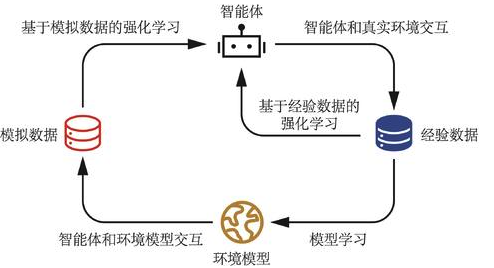
\includegraphics[width=0.88\linewidth]{pic/RL6/基于模型的强化学习方法}
    \caption{基于模型的强化学习方法}
\end{figure}

\begin{algorithm}[htb]
    \caption{Dyna-Q}
    \begin{algorithmic}
        \State 初始化 $Q(s,a)$, 初始化模型 $M(s,a)$
        \For{序列 $e=1\to E$}
            \State 得到初始状态 $s$
            \For{$t=1\to T$}
                \State 用 $\epsilon-$greedy 根据 $Q$ 选择当前状态 $s$ 下动作 $a$
                \State 得到环境反馈 $r,s'$
                \State $\displaystyle Q(s, a) \leftarrow Q(s, a) + \alpha \left[ r + \gamma \max_{a'} Q(s', a') - Q(s, a) \right]$
                \State $M(s,a)\leftarrow r,s'$
                \For{次数 $n=1\to N$}
                    \State 随机选择一个曾经访问过的状态 $s_m$
                    \State 采取在 $s_m$ 下执行过的动作 $a_m$
                    \State $r_m, s'_m \leftarrow M(s_m, a_m)$
                    \State $\begin{aligned}
                         Q(s_m, a_m) \leftarrow & Q(s_m, a_m) + \alpha \left[ r_m \right. \\ & \left.+ \gamma \max_{a'} Q(s'_m, a') - Q(s_m, a_m) \right]
                    \end{aligned}$
                \EndFor
                \State $s\leftarrow s'$
            \EndFor
        \EndFor
    \end{algorithmic}
\end{algorithm}





Dyna-Q 使用 Q-planning 方法来基于模型生成模拟数据, 然后依据模拟数据和真实数据一起改进策略. 

Q-planning 每次选取一个曾经访问过的状态 $s$, 采取一个在此状态下执行过的动作 $a$, 通过模型得到转移后的 $s', r$, 并根据这个 $(s,a,r,s')$, 用 Q-learning 更新动作价值函数. 

每次与环境交互执行一次 Q-learning 之后, Dyna-Q 会做 $n$ 次 Q-planning. 需要注意, Dyna-Q 执行在离散且确定的环境中. 